% This file is based on the "sig-alternate.tex" V1.9 April 2009
% This file should be compiled with V2.4 of "sig-alternate.cls" April 2009

\documentclass[12pt]{article}  %article

\usepackage{url}
\usepackage{color}
\usepackage{enumerate}
\usepackage{balance}
\usepackage{pdfpages}
\usepackage{listings}

\title{Neural Networks and Machine Learning \\ { \large Project 1, Part A: Data preparation}}
\author{
Robert McCartney, Jie Yuan, Sagar Barbhaya
}
\begin{document}
\maketitle

\section{Specification}
\label{Specification}
The goal of this project is to apply neural network models to the recognition of offline handwritten characters. This has been an active application of neural network research for many years, evaluated most famously on the MNIST \cite{website1} data set of handwritten Arabic numerals 0-9. However, we have obtained a set of handwritten characters in several Indian languages provided by the Pen and HW Group of HP Labs in India \cite{website2}, and we would like to evaluate whether the neural network methods which have seen success on differentiating digits in the MNIST data set also perform well on characters of other languages. These data comprise around 100 characters from each of three different languages spoken in India: Tamil, Talugu, and Devnagari. The number of instances for each character in each of these languages ranges from around 270 to 500 examples. Thus our data for this project comprise four unique data sets: the entirety of the MNIST corpus, as well as a distinct corpus for each of the three Indian languages.
The last usage of these data appears to have been in the IWFHR 2006 Online Tamil Handwritten Character Recognition Competition, according to the host website. Though the winning groups are not shown on the website, the best recognition accuracy achieved using these data was 93.53 percent \cite{website3}, well below the accuracy rates achieved for modern neural network models, such as convolutional neural networks and restricted Boltzmann machines. Our primary goal is to apply these newer methods, which have reached accuracy rates below 1\% on the MNIST data set in recent years, to these three Indian language data sets, to determine whether a higher accuracy rate than the IWFHR 2006 winner can be achieved. In addition to these tests, we will also run recognition tests on the MNIST data set, to confirm that our code performs similarly to established methods that achieve high accuracy.
The ultimate goal of our analysis will be first to process and train the MNIST data set and test it against provided MNIST test data, to confirm that accuracy rates are similar to those in published work. Next we will train a single model on all three Indian language character sets, and test using subsets of characters from all three languages simultaneously, to test first whether a useful classifier can be built from these data, and second whether this classifier is effective in discriminating between different languages in addition to different characters of the same language.

\begin{figure}[htb]
\label{tel}
\begin{center}

\includegraphics[width=2in]{telugu.png}
\caption{Example of pre-processed Telugu characters}
\label{tel}
\end{center}
\end{figure} 

\section{Feasibility and analysis study}
\label{Feasibility and analysis study}
We selected handwriting recognition because in recent years, image-based recognition problems have served as the foundation for many novel advancements in neural networks, such as the popularization of convolutional neural networks \cite{website1}, as well as the development of new designs such as deep belief networks. As machine learning students, we believe it would be a great learning opportunity to study many of these newer trends, and this project is a great opportunity to first replicate and then make improvements to the underlying code of the models presented in these papers.

Additionally, we believe that among image-based recognition problems, handwriting recognition is perhaps the simplest and thus most manageable problem, which serves as a good introductory project for experimenting with these models. Other common problems include classifying color images into those that contain cars, or animals, or planes, such as the famous CIDAR data set: these scenarios introduce another level problems including the treatment of pixel values in the three RGB dimensions, as neural network input nodes cannot usually accept multidimensional input, as well as the high variability of the classified objects including views from different angles, different lighting conditions, and variations in the shape and dimensions of the objects themselves. In comparison, handwriting recognition presents a more contained problem in which roughly the same symbol is represented across training examples, the symbol exists solely in 2 dimensions rather than an image projection of a 3-dimensional scene, and the images are grayscale, allowing for pixel intensity values to be directly fed into the neural network inputs.

\begin{figure}[htb]
\label{dev}
\begin{center}
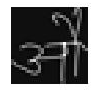
\includegraphics[width=2in]{devnagari.png}
\caption{Example of pre-processed Devnagari characters}
\label{dev}
\end{center}
\end{figure} 


We believe that image recognition problems are particularly exciting, because the images themselves are readily classifiable by human eyes. For example, if two characters are routinely misclassified, we could immediately visualize them side-by-side, and judge the features that are responsible for the misclassification. In most other data sets are are simple lists of attributes, this analysis is very difficult, and since neural networks themselves are difficult to analyze piece-by-piece to justify why classifications are assigned a certain way, a thorough analysis of a model’s classification behavior may be impossible. 

Additionally, because the features comprise pixels in an image, this allows for a reasonable assumption that all pixels and thus all features are potentially relevant for classification. The pixel intensity values can serve as direct input into the neural network input layer, one pixel per input, and no complex preprocessing is required. This also makes possible the implementation of methods aside from neural networks, in case we need a simplistic benchmark against which to test our models. For example, a very simple model may involve a Euclidean distance calculated against all pixel pairs between two images, to get a rough estimate of how similar they are. In many other data sets, the attributes may have different magnitude scales or ranges, or be either continuous or discrete, or be measuring completely different forms of information that are inappropriate for direct comparison as in the image case. 
We selected the 3 Indian language data sets and the MNIST data set largely because these were the only sources which provided readily-accessible handwriting data. Many of the other sources that we investigated, including a Chinese character data set, required submission of a request to the authors for them to approve sharing of the data, and in some cases there were fees attached to acquiring data. We also found these three data sets advantageous because they come from the same organization, so their file structure and image types are roughly the same, which simplifies our preprocessing steps.

The tools we will use will largely be in Matlab. This is because image manipulations are much simpler in Matlab than in other languages, and one of our main bottlenecks will be in processing a large number of images. Additionally, many neural network operations can be generalized into matrix calculations, which are quite fast and elegant, especially in Matlab. For these reasons many implementations of newer neural network models, namely those applied to the MNIST data set, are done in Matlab, and this allows us to use their code as a starting point to conduct our own analyses. 

Regarding specific models, we will experiment mainly with convolutional neural networks and restricted Boltzmann machines. The use of convolutional neural networks is optional - commonly the pixels are directly input into a neural network, one pixel per input. The convolutional neural network can be run on the pixels themselves, and produce an output that is then fed as input into the main neural network classifier, or classified using an SVM or other vector classification method[cite]. This potentially offers advantages such as identifying characters even when there are differences in their location or rotation within the image. Restricted Boltzmann machines have emerged recently as very efficient generative models for classifying images, and we would like to use these mostly because this is a current trend in machine learning, and because we have obtained code from papers that have applied this successfully to MNIST data \cite{website4}. One other useful feature is that because the visible layer of RBM’s pertain directly to the input pixels, the weights of the hidden nodes to visible nodes can themselves be visualized as images, where pixels of high weights indicate that a given hidden node's activation is highly sensitive to that pixel’s input. We think this would be a cool thing to visualize.  


\begin{figure}[htb]
\label{mnist}
\begin{center}

\includegraphics[width=2in]{MNIST.png}
\caption{Example of pre-processed MNIST digits}
\label{mnist}
\end{center}
\end{figure} 

\begin{figure}[htb]
\label{tamil}
\begin{center}
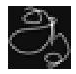
\includegraphics[width=2in]{tamil.png}
\caption{Example of pre-processed Tamil characters}
\label{tamil}
\end{center}
\end{figure} 


\section{Implementation}
\label{implementation}

The data were downloaded from the aforementioned sources and unzipped into a Matlab directory. The MNIST data comes with a provided converter for extracting the data from the zipped files and saving them as .ascii files (converter.m). Within the ascii files, each 2D matrix representing an image is flattened into a single vector, and every row contains one vector pertaining to one image. All images are 28x28 pixels. In order to make these images compatible with the other data sets, we decided to normalize all of the pixel intensities within these .ascii files by subtracting the mean intensity in each image from each pixel, and dividing by the standard deviation of the intensities of the image. This is done in the first section of our overall preprocessing script.
  
The next step was to extract the the image files from the three Indian languages data. Within these data sets, the data is divided by user, and within each of these user folders the full set of gestures in .tiff image files is saved. The second part of our preprocessing script traverses all of these user folders for each language, and extracts the .tiff files and reads them into Matlab as images. This creates a matrix representation of the images as before. However, since these images are much higher resolution than the MNIST images, they were resized to 28x28 using the matlab reshape command, allowing the same number of inputs to be used in the neural network. Lastly, the image matrices were flattened into vectors and appended to a matrix, which is eventually saved to a .ascii file as before. One ongoing issue that we are trying to resolve is that the images are organized by class as in the MNIST data set, but by user, which makes creating individual .ascii files for each character difficult. Currently, we generate a single .ascii file for all of the characters in a given language. We may experiment with writing a shell script to reorganize the file structure to make possible the separation of the individual characters into individual files.
Ultimately, the data contained in these images is a set of 28x28 grayscale pixels.  Figures \ref{tel} through \ref{tamil} display examples of 28x28 character images from each of the four datasets, resulting from these preprocessing steps. These are inputted into the neural network or convolutional preprocessing neural network as one pixel per input. Thus the number of inputs for our neural network will be 784, if the pixels are input directly, or smaller if a convolutional network is applied beforehand, which will condense some of the images and result in a smaller input space. The outputs of the neural network will consist of one output node per class, so that under ideal circumstances for a given input character only one output node will activate, and the others will output 0. This is the simplest design because the resulting classification is just the maximum of the output components; however, we will have to experiment on whether this is still sufficient for larger vocabularies, as in our case using three language sets. Regarding division into training and test sets, we would like to first divide the data set by character, so that all characters are represented in the model. Next for each character class, k-fold cross-validation will be used, in which the training examples are divided into k groups at random. Each k is then set aside as a test set, and the remaining groups are used as the training set. The performance across all k test sets for each character can then be averaged. 


\bibliographystyle{abbrv}
\bibliography{termpaper}

% You must have a proper ".bib" file
%  and remember to run:
% latex bibtex latex latex
% to resolve all references
\balance
\end{document}








